\documentclass[tikz,border=10pt]{standalone}
% Scale s = 0.01626 cm/px; origin at ink-centre (282.5, 153.5) px
\begin{document}
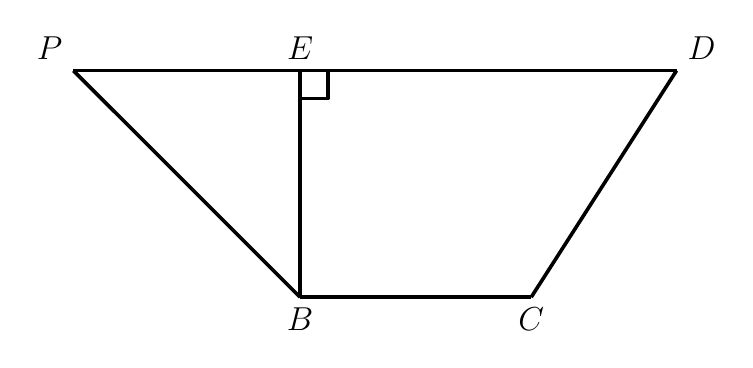
\begin{tikzpicture}[line width=1.3pt, line join=round]
  % Named coordinates (converted from pixels, y flipped)
  \coordinate (P) at (-3.830,  1.439);
  \coordinate (E) at (-0.951,  1.439);
  \coordinate (D) at ( 3.830,  1.439);
  \coordinate (B) at (-0.951, -1.439);
  \coordinate (C) at ( 1.984, -1.439);

  % Main segments
  \draw (P) -- (E) -- (D);   % top edge P-D through E
  \draw (P) -- (B);          % P-B
  \draw (E) -- (B);          % E-B (vertical)
  \draw (B) -- (C);          % B-C
  \draw (C) -- (D);          % C-D

  % Right-angle mark at E (side about 0.355 cm, inside corner ED/EB)
  \draw (-0.596, 1.439) -- (-0.596, 1.084) -- (-0.951, 1.084);

  % Labels
  \node[above left,  font=\fontsize{13}{15.6}\selectfont] at (P) {$P$};
  \node[above,       font=\fontsize{13}{15.6}\selectfont] at (E) {$E$};
  \node[above right, font=\fontsize{13}{15.6}\selectfont] at (D) {$D$};
  \node[below,       font=\fontsize{13}{15.6}\selectfont] at (B) {$B$};
  \node[below,       font=\fontsize{13}{15.6}\selectfont] at (C) {$C$};
\end{tikzpicture}
\end{document}